\documentclass[12pt]{article}
\usepackage{graphicx}
\usepackage{setspace}
\usepackage{underscore}
\usepackage[margin=1in]{geometry}	% Page margins
\usepackage[]{natbib}
\doublespacing
\begin{document}

\author{Samuel Leeman-Munk}
\date{\today}
\title{The Dual-Prolog Natural Language Database \\ with Procedural Frontend}
\maketitle
\abstract{A Natural Language Queriable Database is a collection of knowledge that a user can gain knowledge from much like he or she might ask another human being. Although the ultimate vision of a Natural Language Database (NLD) is still in the realm of science fiction, Natural Language Databases of varying ability do exist today, and many other well-known software such as Google and Wolfram Alpha use Natural Language techniques in helping their users get what they want.

Prolog is a declarative logic programming language associated with both Natural Language Analysis and Artificial Intelligence, making it a prime candidate for both parsing natural language queries and finding answers to them. This paper discusses a theoretical NLD that uses two Prolog databases: one English language parsing database and one database of information. These databases are connected with an imperative front-end, in this paper Perl.}
\clearpage
\section*{Introduction}
Imagine 24-hour customer support with no hold time. Consider a doctor's office that can advise and assist at a professional medical level thousands of people at once. Think if instead of fumbling around on Google trying to get just the right search term, you just ask a question and have it instantaneously answered. Imagine a computer that is smart enough to tell you exactly what you want to know, rather than simply what you ask. These are the ultimate visions of the Natural Language Queriable Database. Unlike conventional databases that are accessed using algorithmic computer languages, a Natural Language Database (NLD) handles the translation from human language to computer language itself, allowing people with no technical skill to ask questions and get helpful answers.

Prolog, short for Programmation en Logique (programming in logic) was developed in the early 1970s as a processor for the French language, but has since become a language associated heavily with both natural language processing and artificial intelligence ~\citep{birthofprolog}. For this reason, Prolog seems a particularly elegant solution to an Natural Language Database, which uses both natural language processing and artificial intelligence in the process of understanding a question a user asks and finding the answer to that question. This paper explores the subjects of the Natural Language Database and Prolog in general, and specifically explores a Natural Language Database for English speakers that employs a procedural frontend connecting two Prolog programs -- one for natural language processing and one for intelligently finding answers to the disambiguated queries.

\section*{Algorithmic Language Parsing}
Unfortunately, translating even the simplest human question into something a computer can understand is non-trivial at best. Human languages are notorious for exceptions and inconsistencies that do not fall easily into algorithmic parsing. Linguistic anomalies, ambiguous questions, improperly formed questions with misspellings and grammatical errors, poorly worded questions, statements that imply questions, and questions that may in fact want something different from what they literally ask plague attempts at computationally understanding what a human asking a question really wants to know ~\citep{Jurafsky}.

For the above reasons, it seems to the casual observer that language recognition cannot be subjected to a deterministic process ~\citep{Marcus}. Indeed it's reasonable to believe that no algorithm of any complexity could have a 100 percent success rate communicating with humans - even humans fail to understand human speech now and then. An algorithm must make educated guesses as to the meaning of a human request, the accuracy of the guess increasing with the sophistication of the algorithm. Fortunately, despite their algorithmic shortcomings, natural human languages do have forms and structures that to a limited extent can be parsed into logical meaning. For a parser to understand the meaning of a human question as completely as possible, this is where to start.

The first logical step in making a language parsing algorithm is to separate the words into logical groups. Of course, the first and most appropriate grouping for natural language is parts of speech. Far more than merely the grade-school noun, verb, adjective, article, interjection and a few more, scholarly part-of-speech lexicons segregate words into many fields. From Penn Treebank's 45 to a staggering 146 in the C7 tagset, there's some disagreement as to exactly where one type of word ends and another begins. ``Tagging'' words with their parts of speech is the first step for syntactic language recognition, as part of speech more than anything else allows for predicting how words will fit together in a sentence and provides tremendous help in disambiguating word meaning ~\citep{Jurafsky}.

There are two supercategories of parts-of-speech: closed class and open class types. A closed class is one that is comparatively less likely to accept new members.  New prepositions, for example, are exceptionally rare in comparison to an open class part of speech such as nouns and verbs, which constantly accept new members, often borrowed from other languages (restaurant from French) or brought from other parts of speech ('to google'). Between spoken dialects and bodies of text, the set of open class words can vary dramatically, but large enough samples tend to share closed class words ~\citep{Jurafsky}. 

Open class types tend to hold the bulk of a sentence's meaning while closed class types tend to be "function words" that serve as abstract qualifiers and grammatical glue that holds the other words together. As an example of subdivisions in part of speech, Daniel Jurafsky and James H. Martin's \underline{Speech and Language Processing} divides the function words into prepositions(under, beside), articles(a, an, the), pronouns(she, his, what), conjunctions(and, but) auxiliary verbs(can, should, will), particles(down, off), and numerals(one, fifteen). Open class words tend to be nouns, verbs, adjectives and adverbs, each of which is further subdivided to varying extent depending on the opinions of the divider ~\citep{Jurafsky}.

Unfortunately, one word can exist in multiple parts of speech, and even with a completely divided and subdivided dictionary, it's generally not trivial to tag any given sentence. "Watch," for instance, can refer to a handheld timetelling device or someone's turn to stand guard, or it can refer to observing something over a period of time. "Watch my watch," could be noun-pronoun-noun, noun-pronoun-verb, verb-pronoun-noun or verb-pronoun-verb. Here an algorithmic parser can use a predefined set of rules to pick the most likely part of speech. For example, watch can be either a main verb or a count noun, a non-proper noun that refers to a distinct object rather than a mass, such as water. Singular count nouns don't tend to begin sentences as they tend to follow an article so the watch at the beginning of the sentence is more likely a verb. This reduces the possibilities to verb-pronoun-verb or verb-pronoun-noun. "My" is a possessive pronoun, which tends to precede a noun (that which is possessed), so verb-pronoun-noun is the most reasonable interpretation.  Working with text by way of picking words and phrases based on the one preceding them is known as a Markov chain algorithm ~\citep{Markov}.

Tagging requires a ruleset, and different styles of tagging are separated by how the rules are decided. A Rule-based tagger gets its rules from a vast manually assembled database, while a stochastic tagger makes a table of rules from analyzing an already-tagged corpus of text ~\citep{Jurafsky}. While the former tends to be more reliable, it does not scale well. Manually encoding every grammatic possibility of the English language can become costly and time consuming. The latter can analyze a large corpus of text, but the corpus must already be tagged, which, except in the unlikely situation that another high-quality tagger is available, must also be done manually. In a Natural Language Database environment, a manually encoded ruleset that covers the most commonly used structures is sufficient. A full-featured NLD has other failsafes that can account for unrecognized grammars. 

Sometimes after the Markov Chain tagging process a word still has multiple possibilities. In this case, the word can have more than one tag ~\citep{Tomita}. This is clearly not preferable, and cannot be disambiguated without moving to a higher level of understanding. This new level of understanding will also help get meaning from complex sentences. A sentence like ``I really think that Tyler should start on that big project soon,'' contains structures poorly represented by just a list of parts of speech. We can move closer to solving the problem of ambiguity of individual words while also gaining an entirely new level of meaning by identifying entire phrases that behave as a particular word type in a group ~\citep{Jurafsky}. For instance, The above sentence nagging Tyler could be described in terms of the parts of speech of each of its lowest components, or at a higher level, it could be marked "noun phrase(I) verb phrase(really think) conjunction(that) noun phrase(Tyler) verb phrase(should start on that big project soon)." In fact, it could be marked any number of ways. The last big chunk could be split into smaller verb and noun phrases, the first parts could be put together, ``I'' could be separated as one noun phrase while the rest of the sentence gets lumped together into a verb phrase, or the whole sentence could just be marked ``sentence.'' The mathematical system for modeling phrase structures in this way is called ``Context-Free Grammar'' or more intuitively ``Phrase-structure Grammar'' ~\citep{Peters}. The specific rules for grammatical phrases differ depending on what list of part-of-speech tags is being used, but every proper system ends at the same result.

Naturally, just marking a sentence ``Sentence'' isn't particularly helpful. Separating it entirely into its lowest parts is moreso, but only marginally.  One option is to try and find a middle ground with the most meaningful possible structure, but what might be a better option would be to store all the levels, say, in a tree (\ref{fig:Phrase-Tree}). This system provides a more sophisticated level of understanding of sentence structure, and provides better information to help a parser derive useful meaning. For instance, three levels up from the bottom of the tree we can see the sentence as a noun phrase followed by a verb phrase, a form generally taken by declarative sentences. Similarly, ``Watch my watch'' maps out to be just one big verb phrase, suggesting an imperative statement, which a natural language database can then parse to find out if it can do what the user has told it to do~\citep{Jurafsky}. 

\begin{figure}[p]
	\centering
		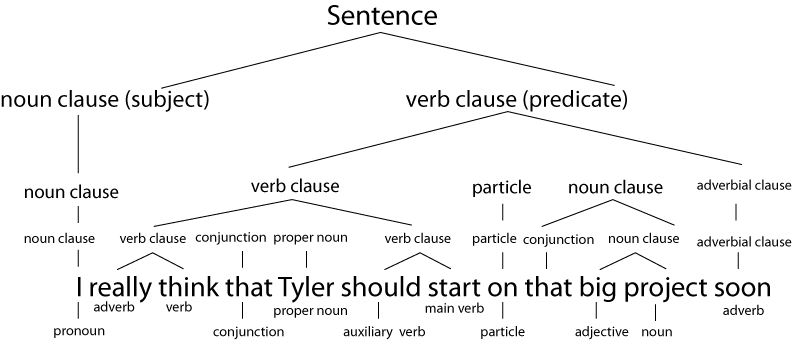
\includegraphics[width=13cm]{Phrase-Tree}
		\caption{One example of a parse tree}
	\label{fig:Phrase-Tree}
\end{figure}

It's a little more complicated to find a parse tree in a sentence than it is just to go through and tag word-by-word. The process can be thought of as a search algorithm that searches through the set of all possible trees to find the one that fits the sentence. We start knowing that the leaves at the bottom of the tree must be all of the words of the sentence in order, and that top of the tree must be a sentence, which breaks down in a certain fashion defined by the grammar of the language ~\citep{Jurafsky}.

There are two basic algorithms behind the parsing of sentences into parse trees. The first starts from the root node, the sentence, and works down, expanding through each possible expansion of a sentence, then recursively expanding each of the resulting partial trees through all their possibilities, until reaching the part-of-speech categories at the end. Then the resulting part-of-speech category sets are checked, and any that don't match the sentence are thrown out. The remaining trees (ideally tree) are the sentence's parse trees. Understandably, this is called the top-down algorithm. The second algorithm, the bottom-up algorithm, starts from the words and their tags themselves, and follow the rules backwards. Trees that make it to sentence are kept as parse trees and the rest are tossed. In both cases, ambiguous sentences that return multiple parse trees can be disambiguated by linguistic heuristics or selected later by whether the artificial intelligence section of the database thinks they make sense. ~\citep{Tomita}

The top-down tree and the bottom-up tree each have their strengths and weaknesses. A strictly bottom-up algorithm can take the input and build partial trees that cannot even fit with their immediate neighbors, let alone the sentence at the top, while a strictly top-down algorithm generates all the trees that can possibly be made by the grammar before even looking at the input. Neither of these approaches takes complete advantage of both the grammars and input words ~\citep{Jurafsky}.

Most modern parsers use a combination of the top-down and bottom-up approaches. For example, by looking at the left corner, or the leftmost leaf of the tree, i.e. the first word of the sentence, we can cancel certain sentence types from the start, dramatically reducing the number of trees a top-down parser will need to search through. ``I really think that Tyler should start on that big project soon,'' starts with ``I,'' a pronoun, which can only be the start of a noun phrase, meaning the sentence cannot take the Verb phrase form of imperative, nor can it start with an auxiliary verb (can,should) to form a yes-or-no question, so those and other similarly ill-fitting trees can be cut out before expanding, reducing the workload by more than two thirds ~\citep{Jurafsky}.

The simple CFG-based grammar as we have described it does not cover grammatical agreement. A grammatical detail as minor as the difference between ``he eats'' and ``he eat'' would at a glance not seem to bear particularly heavily on language comprehension and understanding, but Manny Rayner et al. conducted a study in 2000 suggesting just the opposite. Rayner found that CFG-based English language recognition in two separate systems had a significantly lower rate of semantic error when taking into account grammatical agreement ~\citep{Rayner}.

A CFG-based grammar can be designed to cover grammatical agreement, but it would require making a new phrase for each combination set of agreements. A simple verb clause would need to be expanded into a singular past verb clause, a singular present verb clause, a singular infinitive verb clause, a plural past verb clause and so on, and that's not even taking mood into account. For this reason, we can use a more compact formalism based on the CFG, a Definite Clause Grammar (DCG) works very much like a CFG except that a clause can have multiple variables in addition to its identifier. A verb clause, then, has values denoting its mood, tense, and number, that affects the valid moods, tenses, and numbers of its sub-clauses. DCGs also introduce context-dependency and allow for even better translation into meaning. DCGs have been used to make many language parsing algorithms for both natural languages and programming languages ~\citep{DCGNLA}.

\section*{The Dual-Prolog Natural Language Database}

The Dual-Prolog Natural Language Queriable Database seeks to take advantage of Prolog's two strongest features by using two Prolog components that are accessed using a Perl frontend. In this section we will discuss how the system works as well as explaining why Prolog works so well in both contexts.

\subsection*{The Prolog Natural Language Parser}

Prolog's relationship with DCGs is hardly a new one. In fact, it's difficult to mention one without the other coming up, especially in the context of natural language analysis. Prolog handles DCGs natively, and has built-in algorithms for making parse trees from them, making it an excellent choice for natural language analysis. A Prolog natural language analyzer can go through a sentence and print out a parse tree, which another program (such as the Perl frontend) can read and translate into a Prolog database command to be sent to the Prolog knowledge database.

The Prolog Natural Language Parser (NLP) consists of two linked Prolog files. One is a file of DCG grammar rules, and the other is the vocabulary list of terminal nodes, which represent English words. These two files work directly with each other as one component and do not require the assistance of the Perl frontend. The vocabulary and grammar are kept separate to free the relatively flexible and expandable vocabulary from the more rigid grammar rules, making both easier to maintain.

Each word in the vocabulary is accompanied in its node by appropriate indicators for managing agreement and other small grammatical details. For instance, verbs are accompanied by a list of complement types that must follow them. 'sleeps,' for example, works well on its own, or can take a preposition clause. ``sleeps'' is a valid verb clause, but ``sleeps a cat'' is not. ``Sleeps'' gets a list [] to indicate that it does not have any special complement requirements. ``Give,'' on the other hand, can be followed by two noun phrases, ``Give Andrew a dollar,'' or just one noun phrase, ``Give a dollar,'' so its list is [np,np],[np] ~\citep{PS}. 

Because a significant portion of my Prolog parser is based on their work, I would like to note here that Pereira and Sheiber, in their book \underline{Prolog and Natural Language Analysis}, suggest a more compact method of notation for words. Pereira and Shieber recommend that a word be defined as all of its inflections, placed in a predetermined order representative of the grammatical placements. In this scheme, ``apple'' could be represented as ``np(apple,apples)'' where the first place indicates the singular, and the second the plural ~\citep{PS}. I have made a conscious decision not to use this method because it makes it difficult to automatically add new words. Assuming the vocabulary should be able to expand dynamically, whether in the process of reading queries or through separate analysis of corpus text\footnote{This is further discussed in the subsection entitled ``Dynamic Vocabulary Building'' at the end of this section}, the encoding of a word cannot require foreknowledge of all of that word's forms, as for the most part only one form will be seen at a time in any given sentence. So, at the expense of a less concise notation, we have greater flexibility in defining the words that make up the DCG terminal statements.

The grammar file contains the non-terminal statements and everything therein. While the vocabulary is comparatively simple, the grammar is where most of the hard work happens, and where Prolog's strengths and weaknesses start to become more important.

By default, Prolog parses DCGs and CFGs from the top-down, going left-to-right, and depth-first, meaning it follows a node down to its terminal before moving on to the next node. This works well for encoding languages, except it can run into a problem in a case where a sentence can expand into a potentially infinite number of clauses, which is the case in English. An intuitive way to describe to Prolog a situation like, say, an adjective phrase with any number of adjectives might be to say \[AdjectivePhrase \rightarrow adjective\] \[AdjectivePhrase  \rightarrow adjective\mbox{ }AdjectivePhrase.\] In attempting to parse this, Prolog would expand the adjective phrase into an adjective phrase and adjective. Then it would expand this new adjective phrase, making another adjective phrase to expand, and so on, never completing ~\citep{leftrecursion}. 

Fortunately, although English has the potential to, say place an infinite number of adjectives in front of a noun, a common sentence generally has no more than two or three. It would be reasonable to only check for adjectives out to five, or to be safe, ten. Writing naturally, an English speaker is extremely unlikely to need anywhere near ten adjectives in front of any one noun. The same goes for all clauses, although it may be prudent to give different clauses different limits.

A Prolog natural language parser could handle this limitation of clauses in one of two ways: it could make a separate expansion rule for each number of adjective clauses, or it could take advantage of Prolog's special relationship with DCGs. Beyond the normal capabilities of DCGs, Prolog can embed arbitrary commands into nonterminal nodes ~\citep{PS}. Here is one place Prolog dabs in procedural language as opposed to its normal declarative style. Continuing with our adjective example, we can give the adjective phrase a variable that starts at zero for the first occurrence, but an adjective phrase child of that adjective phrase increments the variable by one. Then its child increments it again, etcetera until at ten the function embedded in the adjective phrase only allows its phrase to expand to a terminal adjective, ending the recursion. 

As you can imagine, the usefulness of Prolog's ability to extend DCGs with arbitrary code doesn't end there. Mostly my database would just use it to speed the parsing of trees, like the example presented in the Algorithmic Language Parsing section of thinning the list of possible trees based on the first word in a sentence. Tree parsing is where most of the computation time in a natural language parser goes, so that in and of itself is worth the effort of designing special DCGs.

My Prolog Natural Language Parser handles the first step in parsing a sentence into meaning. It converts a sentence into a parse tree using a list of words and grammar rules as well as Prolog's built-in tree-finding algorithms. To help along the potentially time-consuming process of tree parsing, the parser takes advantage of Prolog's ability to augment DCG grammars with arbitrary code.

\subsection*{The Prolog Intelligent Database}

The Prolog Intelligent Database is so named because in addition to being able to handle queries that ask for specific pieces of information, it can use a certain amount of intelligent reasoning to use the information it does know to give an answer not directly stored in its database. In official terms, it is an ``expert system''. Besides natural language parsing, Prolog is also well-known for its use in expert systems. An expert system is important in the Dual-Prolog NLD so that the user can get the right answer even if he or she asks a roundabout question.

It should be no mystery why Prolog is well-suited to the task of being an expert system. You may remember from earlier that Prolog is short for programming in logic. Prolog is in fact in and of itself already a sophisticated inference engine. All a Prolog programmer has to do is give Prolog a set of rules and definitions and Prolog's algorithms handle the rest. An explanation of how Prolog's logic algorithms work follows as I explain how the knowledge database in the Dual-Prolog NLD is encoded and the nature of a user query by the time it gets to this stage.

To explain how the Prolog Intelligent Database works, I'll use an example database containing simple information about the Earlham Computer Science Department, although in fact the database I propose is a general one, and the techniques used can be applied to many different bodies of knowledge with minimal modification. We can start with a tree showing a couple of the Computer Science (CS) classes (or classes required for a CS major) each teacher is known to teach, as well as a subset of the students in each class and some information about these students. These trees constitute the basic data in this example database, and the rest of this section describes how the Prolog Intelligent Database uses this information to infer useful answers to what are called ``Goals''. 

Let's start with a simple verification question - one that only requires a ``Yes'' or ``No'' answer, and is directly stored in the database. Say the user asks ``Is Sam a student?'' This would go through the appropriate parsing to become the Prolog goal ``is(sam,student).'' Notice first that Sam is not capitalized now. This is because Prolog interprets terms beginning with capital letters as variables. Spaces also may not occur in Prolog term names, so underscores are substituted. Conflicts that may arise from this (such as if Earlham had a surface to air missle (SAM) program) are handled by assigning term names uniquely. For instance it would be very hard to find another instance best described as samuel_leeman_munk\footnote{The handling of words with multiple meanings is detailed more in The Procedural Frontend}. In this case, though, we can safely use ``sam'' as there are no conflicts. ``is(sam, student)'' is explicitly defined in our set of trees, which Prolog shortly discovers, returning ``Yes.''

Easy enough. Now let's say that we want to know if Programming Languages is taken by Sam. This would be encoded as ``is\_taken\_by(programming_languages, sam).'' The answer is, of course, ``No.''  Then we could ask by whom Programming Languages is taken. Who is what we want to find out, so it is given to the database as a variable. ``is_taken_by(programming_languages,Whom)'' checks to find terms that fit in the variable ``Whom'' and returns ``Whom = Aaron.'' Prolog doesn't care what the variable is called, but, like in any programming language, the programmer appreciates the distinction. Working purely from the existing information in the database, Prolog can already verify claims and answer simple, direct questions. These, however, only account for the most rudimentary of Prolog's capabilities.

Let's try rephrasing the question. ``Who takes Programming Languages?'' or ``takes(who, programming_languages),'' although it is intuitively the same question as before, it is not explicitly described as such in the database, and therefore cannot be answered without a little bit more help. This help comes in the form of a clause that defines ``takes(Who, What)'' as ``is_taken_by(What,Who).'' In Prolog this is written as such:
\begin{center}
takes(Who,What):-is_taken_by(What,Who).
\end{center}
This is exactly equivalent to telling Prolog ``If something is taken by someone, then that someone takes that something.'' We add this one line of code to our Intelligent Database, and Prolog can tell a user who is taking a class either way the question is posed. Accounting for another way of posing this or any other question is as simple as defining another clause.

Say we want to know whether Charlie teaches Sam? Although it again is easily intuitable by a human looking at the tree, the Prolog database does not know that teaching a class taken by a student means that one is teaching the student. We can let our database know this is the case by telling it the following:
\begin{center}
teaches(Who,Whom):-teaches(Who,Class),is_taken_by(Class,Whom).
\end{center}
If someone teaches a class and that class is taken by someone else, the first person is teaching the second. This raises a new problem, however. At this point, asking Prolog to list who Charlie teaches will get not only Aaron and Sam but CS128, Capstone, and Operating Systems all as answers. As mentioned before, ``Who'' doesn't mean anything to Prolog; it's just a variable. Prolog lists all the solutions it finds, the explicit ones as well as the ones specified by our new clause. If we had only the Intelligent Database to work with this would be a serious problem, we would have to cut the explicit links we've relied so heavily upon until now, for one thing. Fortunately, we have more power than just the rules within the Intelligent Database itself, we have a certain degree of power over how the user input is translated into a Prolog goal. Without going into too much detail regarding the Procedural Frontend, we can demand that the terms to fit to a ``Who`` variable meet certain requirements. For example, we can translate ``Whom does Charlie teach'' as ``teaches(charlie, Whom),student(Whom).'' More generally, we can define a new clause in the database:
\begin{center}
person(Who):-is(Who,student).

person(Who):-is(Who,professor). 
\end{center}
Now Prolog knows that both students and professors are people, and all the Procedural Frontend has to do to differentiate ``Who'' from ``What'' is to tack on ``person(Who)'' to the end of a goal.

Another place where the Procedural Frontend helps is handling synonyms of terms. We've handled verb synonyms already. Verb synonyms are easy to make in the database because all applicable terms can be represented at once by using variables. The situation is different for making synonyms of terms, as in Prolog functions cannot be represented by variables. To define a synonym of a term, one would need to define it separately for every applicable function, which would be ugly, tedious to build, and difficult to maintain and read, defeating the purpose of using synonyms entirely. So, the Procedural Frontend keeps a list of words that it maps to database-supported terms, which it uses in the goals it sends to the Intelligent Datbase.

\subsection*{The Procedural Frontend}

As we've seen in the previous sections, the general purpose of the Procedural Frontend is to handle the parts of a Natural Language Database that are ill-suited to Prolog. The Procedural frontend connects the Prolog Natural Language Parser and the Prolog Intelligent Database to each other to and interfaces them to make a user-friendly environment. In general, the frontend takes an English string from the user and sends it to the Natural Language Parser, which creates a parse tree that it sends back to the frontend. The frontend then takes the parse tree and, using structure-to-meaning analysis, translates it into an intelligent database Prolog query, which it sends to the Intelligent Database. The Intelligent Database then sends back an answer which the frontend sends out to the user along with a brief description of what it thought the user was asking.

Let us first handle the situation in which everything happens predictably and as expected. The question uses no unexpected vocabulary and requests unambiguously exactly what the user wants to know, which, as it turns out, is something the Database will be able to tell it. Say we ask the database ``Who works for Charlie?''

\subsubsection*{Cooperative Query Parsing}

This section is likely to be incorporated into The Perl Frontend section. It describes how when my Natural Language Database can't immediately answer a user's question, it can ask for more information or suggest information that it thinks the user meant to ask for. At is most basic, this is a widely implemented concept that is seen in well-known search engine Google as well as knowledge database Wolfram Alpha.

\subsubsection*{Dynamic Vocabulary Building}

English is a gigantic and ever-growing language. Manually constructing a vocabulary database can only account for a fraction of it without becoming cost-prohibitive. A dynamic vocabulary database with a strong manual base could learn new words through analysis of large corpi or could even with cooperative query parsing ask a user to help it understand a word it does not know.

Each of these methods has significant weaknesses. Analyzing large corpi would be feasible for expanding the Language database's vocabulary, but would be much more challenging and error-prone applied to the knowledge database. If it were only applied to the NLP's vocabulary, the NLP could give a tree that the frontend would translate into a query that the Intelligent Database would not know what to do with. Cooperative Query Parsing could ask for a synonym for a word it didn't know until it got a match, but this would be a security risk, as a user could easily provide false vocabulary terms and make the database less effective.

\subsection*{The Dual-Prolog Database in the age of Parallel Processing}

The most computationally intensive portion of the Dual-Prolog NLD would be the Intelligent Database and the NLP. The NLP's tree parsing could likely be parallelized, as could the Intelligent Database, depending on the complexity of the question. I have more research to do on this regarding Prolog's parallelizability specifically.  

\section*{Future Work}

\singlespacing
\bibliography{capstone}{}
\bibliographystyle{plainnat}
\end{document}